\section{Introduction}

\subsection{Numerical Methods compared to Symbolic Methods}

Engineering design for given specifications  often requires the solution of nonlinear systems of equations after defining component element parameters.
%functional specification component parameters. 
Usually for the determination of the wanted variables numeric optimizing procedures are used, which do not function reliably however already for small design problems with a comparatively small number of unknowns. 
Above all, the complexity order of many usual optimizing algorithms is exponentially dependent on the number of variables, which  cause problems  (a problem, known as the {\em curse of dimensionality} \cite{Michalewicz} is), then the selection of suitable initial values, the unwanted finding of locally instead of global optima and the principle-conditioned behavior during the solution of systems of equations with degrees of freedom, with which a uniqueness of the solution vector is not realizable. 

The best procedure for the accomplishment of a design task would basically be a complete analytic solution of the corresponding system of equations. Analytic functions, which describe explicitly the wanted values as functions of the specification parameters, would have to be determined only once and would be available afterwards to the arbitrarily frequent evaluation with modified parameters, e.g. within design data bases of CAD systems. Besides analytic dimensioning formulas clarify qualitatively functional connections between the element values and the specifications and reveal in the relevant cases  the existence of degrees of freedom. 
Since there exists however no generally accepted procedures for the solution of nonlinear systems of equations and in those special cases, in which symbolic solutions can be calculated, the complexity of the results far exceeds by hand calculation to mastering frameworks, the analytic handling of very low dimensioning problems plays so far a subordinated role. 

With the help of modern, efficient computer algebra systems, which are able to manipulate   systems of symbolic equations algebraically, and solve using arbitrary variables, become some of these problem categories nevertheless accessible for an analytic handling. In particular such problems, specified above, which require the solution of linear or multivariate polynomial systems.
Examples of such applications are within many fields of engineering sciences, such as the design of analog electronic circuits, regulation-technical problems, engineering mechanics and robotics \cite{Pfalzgraf}.



\subsection[Examples of Areas of Application of Symbolic Design Methods]{Examples of Areas of Application of Symbolic Design Methods}

On the basis of the following two examples we demonstrate some areas of application of symbolic methods. At the same time, the concrete requirements should be worked out at them, which must be considered with respect to the development of  a universal solution algorithm for symbolic systems of equations .


\begin{example}{TM}

The first example concerns  a simple task  of engineering mechanics. Given is the two rod truss represented in figure \ref{Stabzweischlag}, \cite[S.~112]{Brommundt}, at which under the angle $\gamma$ opposite the horizontals the force $F$ attacks in the point $C$. The rods form the angles $\alpha$ and $\beta$ with the horizontals, the height of the triangle stretched by the rods are denoted with $c$. The  Cross sections  $A_1$ and $A_2$  of the two rods are squares with the side lengths $h_1$ and $h_2$. The modulus of elasticity of the  material used is $E$. 

\begin {figure} [htbp]
\begin {center}
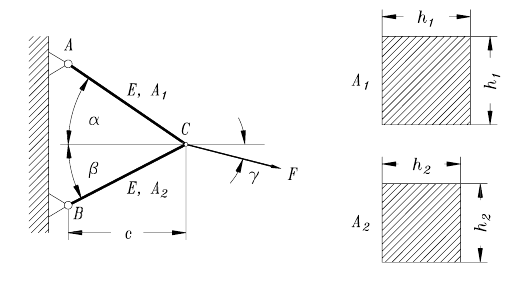
\includegraphics[height=4cm]{zweischl.png}
\caption \protect {\begin {minipage} [h] {10cm}% --- TABLE
Loaded two rod truss (in German: 'Stabzweischlag')
\label{Stabzweischlag}
\end {minipage}
}%small
\end {center}
\end {figure}
%\inbildpsf{Loaded double bar truss}{zweischl.png}{86mm}{Double bar truss}
Due to the load by the force $F$  the truss deforms in such a way, that the point of the triangle in relation to the unloaded status around the vector $(u,w)^T$ shifts, see figure  \ref{Belastung}. On the assumption that the rod lengths variations are small due to the load in relation to the original lengths, now  the cross section dimensions $h_1$ and $h_2$ of the rods are to be determined  in such a way, that for given $F$, $\alpha$, $\beta$, $\gamma$, $c$ and $E$ there results exactly one prescribed shift $(u,w)^T$, i.e. we look for

\begin{equation}
\cvec{a_1\\a_2} = \f( F, \alpha, \beta, \gamma, c, E, u, w).
\end{equation} 

\newpage
\begin {figure} [htbp]
\begin {center}
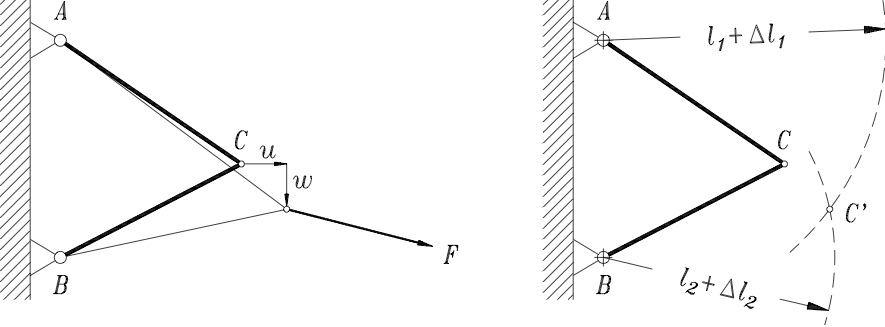
\includegraphics[height=4.4cm]{BELASTG.png}
\caption \protect {\begin {minipage} [h] {10cm}% --- TABLE
Two rod truss elastic displacements
\label{Belastung}
\end {minipage}
}
\end {center}
\end {figure}
%\inbildpsf{Truss elastic deformations}{belastg.eps}{105mm}{Load}

\noindent {\bf Solution:}  From the static equilibrium conditions at the point $C$ it follows after figure \ref{Freischnitt}
\begin{eqnarray}
\sum F_{xi} = 0 & \Longrightarrow & 
  F \cos \gamma - S_1 \cos \alpha - S_2 \cos \beta = 0, \label{TMGS1}\\
\sum F_{zi} = 0 & \Longrightarrow & 
  F \sin \gamma - S_1 \sin \alpha + S_2 \sin \beta = 0.
\end{eqnarray}

\begin {figure} [htbp]
\begin {center}
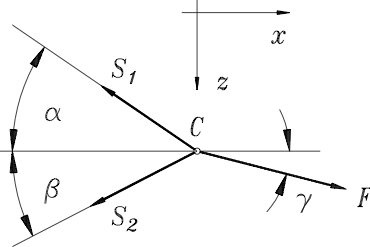
\includegraphics[height=4.4cm]{KRAEFTE.png}{Free body diagram}
\caption \protect {\begin {minipage} [h] {10cm}% --- TABLE
Equilibrium of forces at point $C$
\label{Freischnitt}
\end {minipage}
}%small
\end {center}
\end {figure}

%\inbildpsf{Equilibrium of forces at the point $C$}{kraefte.eps}{44mm}{Free body diagram}

\noindent 
The material equations for the variations of the rod lengths are
\begin{eqnarray}
\Delta l_1 &=& \frac{S_1 l_1}{E A_1}, \\
\Delta l_2 &=& \frac{S_2 l_2}{E A_2},
\end{eqnarray}
whereby for the rod lengths $l_1$ and $l_2$ and for the cross-section areas $A_1$ and $A_2$ we have
\begin{eqnarray}
l_1 &=& \frac{c}{\cos \alpha} \label{l1} \\
l_2 &=& \frac{c}{\cos \beta}  \label{l2} \\
A_1 &=& h_1^2, \\
A_2 &=& h_2^2.
\end{eqnarray}


\begin {figure} [htbp]
\begin {center}
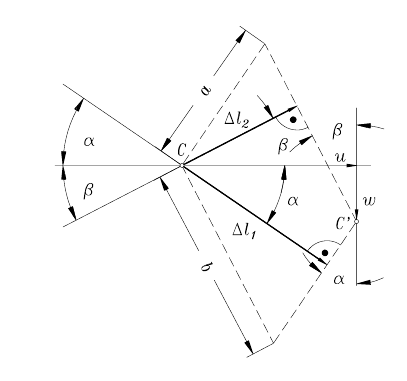
\includegraphics[height=6.4cm]{vschplan.png}
\caption \protect {\begin {minipage} [h] {10cm}% --- TABLE
Displacement plan
\label{Verschiebungsplan}
\end {minipage}
}%small
\end {center}
\end {figure}
%\inbildpsf{Displacement diagram}{vschplan.eps}{60mm}{Displacement diagram}

In the displacement diagram, drawn in figure \ref{Verschiebungsplan}, we replaced the circular arcs, on which the rod ends can move,  by the  tangents perpendicular to the  original rod directions. This is possible, because of the small geometry variations. For the side lengths of the dashed parallelogram we have 

\begin{eqnarray}
a &=& \frac{\Delta l_2}{\cos(90^\circ - \alpha - \beta)}
  = \frac{\Delta l_2}{\sin(\alpha + \beta)}, \\
b &=& \frac{\Delta l_1}{\cos(90^\circ - \alpha - \beta)}
  = \frac{\Delta l_1}{\sin(\alpha + \beta)}.
\end{eqnarray}
Therefore we have for the shifts $u$ and $v$ 
\begin{eqnarray}
u &=& a \sin \alpha + b \sin \beta, \\
v &=& -a \cos \alpha + b \cos \beta. \label{TMGS12}
\end{eqnarray}

The task is now, to solve the symbolic set of equations from the equations  (\ref{TMGS1}) through (\ref{TMGS12}) for the unknowns $h_1$ and $h_2$ explicitly, whereby all unnecessary variables, i.e. $S_1$, $S_2$, $A_1$, $A_2$, $\Delta l_1$, $\Delta l_2$, $a$ and $b$, are to be eliminated.
\end{example}



\begin{example}{ET}

The second example originates from electro-technology and concerns the design of analog electronic circuits. For the two-stage transistor amplifier drawn in figure \ref{BJTAmp} \cite{Nuehrmann}, there are circuit design equations to be determined, which describe the values of the seven resistances 
$R_1 \, \ldots \, R_7$ as function of the operating voltage $V_{CC}$, of the small signal amplification $A$, of the input resistance $Z_i$ and the output resistance $Z_o$  of the circuit for numerically determined operating points of the transistors:
\begin{equation} \label{Rdim}
\cvec{R_1\\\vdots\\R_7} = \f( V_{CC}, A, Z_i, Z_o ).
\end{equation}


\begin {figure} [htbp]
\begin {center}
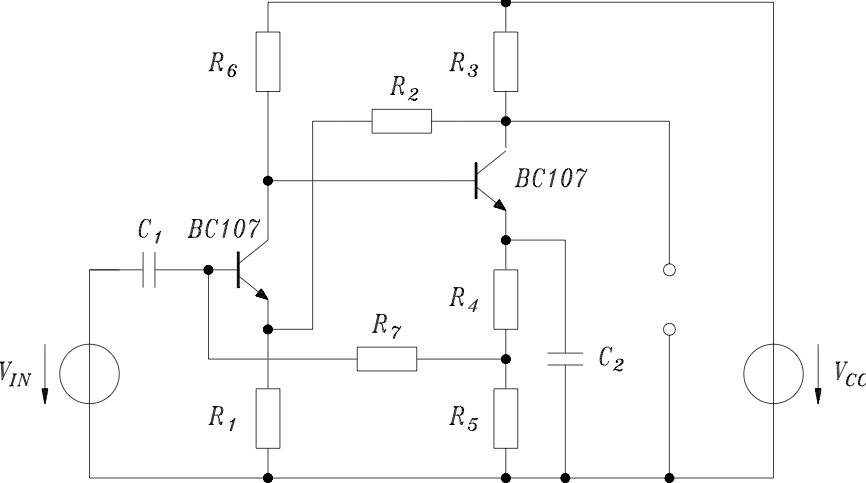
\includegraphics[height=6.4cm]{BJTAMP.png}
\caption \protect {\begin {minipage} [h] {10cm}% --- TABLE
Two-stage transistor amplifier
\label{BJTAmp}
\end {minipage}
}%small
\end {center}
\end {figure}
%\inbildpsf{Two-stage transistor amplifier}{bjtamp.eps}{103mm}{BJTAmp}


\begin {figure} [htbp]
\begin {center}
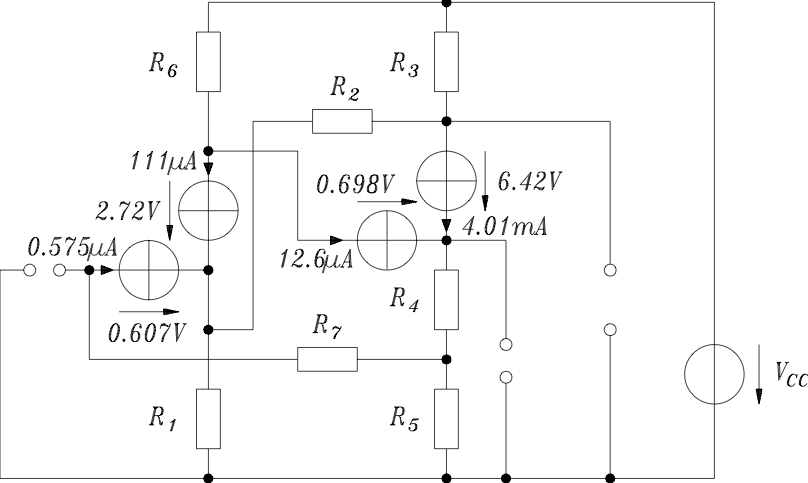
\includegraphics[height=6.4cm]{BJTAMPOP.png}
\caption \protect {\begin {minipage} [h] {10cm}% --- TABLE
Small signal equivalent circuit diagram of the amplifier with specified
transistor operating points
\label{BJTAmpOP}
\end {minipage}
}%small
\end {center}
\end {figure}
%\inbildpsf{Arbeitspunktersatzschaltbild des Verst"arkers mit festgelegten 
%Tran\-si\-stor-Ar\-beits\-punk\-ten}{bjtampop.eps}{96mm}{BJTAmpOP}
For this purpose, with the help of symbolic network analysis procedures \cite{RalfsDiss}  as well as symbolic approximation methods \cite{DA}, 
at first the (highly simplified)  transfer functions $A$, $Z_i$
and $Z_o$ in the pass band of the amplifier are calculated as functions of the element parameters and the operating point values.
\begin{eqnarray}
A   &=& \frac{145303681853 R_2}{145309663773 R_1}\label{BJTAmpA} \\
Z_i &=& R_7\\
Z_o &=& \frac{1675719398828125 \: R_2 \: R_7 
+ 394048139880824192 \: R_1 \: R_2}{136552890630303121408 \: R_1}
\label{BJTAmpZo}
\end{eqnarray}
The values of the resistances $R_1\, \ldots \, R_7$ do not only determine the small signal characteristics, but determine the operating point of the circuit. Therefore the resistances
are to be determined in such a way, that the small signal and the operating point specifications are fulfilled  {\em at the same time}. For this reason, an  extensive sparse tablet set of equations  (\ref{BJTAmpSTA1}) -- (\ref{BJTAmpSTAn}) is added to the equations (\ref{BJTAmpA}) -- (\ref{BJTAmpZo}), which comes out of the small signal circuit diagram of the amplifier represented in figure \ref{BJTAmpOP}.
\begin{eqnarray}
I_{\rm VIN}+I_{\rm C1} & = & 0 \label{BJTAmpSTA1}\\
I_{\rm R7}+I_{\rm FIX2,Q1}-I_{\rm C1} & = & 0 \\
I_{\rm R2}+I_{\m R1}-I_{\rm FIX2,Q1}-I_{\rm FIX1,Q1} & = & 0 \\
I_{\rm R6}+I_{\rm FIX2,Q2}+I_{\rm FIX1,Q1} & = & 0 \\
-I_{\rm R7}+I_{\rm R5}+I_{\rm R4} & = & 0 \\
-I_{\rm R4}-I_{\rm FIX2,Q2}-I_{\rm FIX1,Q2}+I_{\rm C2} & = & 0 \\
I_{\rm R3}-I_{\rm R2}+I_{\rm FIX1,Q2} & = & 0 \\
I_{\rm VCC}-I_{\rm R6}-I_{\rm R3} & = & 0 \\
  \medskip
-V_{\rm VIN}+V_{\rm R1}+V_{\rm FIX2,Q1}+V_{\rm C1} & = & 0 \\
-V_{\rm R2}+V_{\rm FIX2,Q2}-V_{\rm FIX1,Q2}-V_{\rm FIX1,Q1} & = & 0 \\
-V_{\rm R6}+V_{\rm R3}+V_{\rm R2}+V_{\rm FIX1,Q1} & = & 0 \\
V_{\rm R7}+V_{\rm R4}-V_{\rm R2}-V_{\rm FIX2,Q1}-V_{\rm FIX1,Q2} & = & 0 \\
-V_{\rm VIN}+V_{\rm R7}+V_{\rm R5}+V_{\rm C1} & = & 0 \\
-V_{\rm VIN}+V_{\rm R2}+V_{\rm FIX2,Q1}+V_{\rm FIX1,Q2}+V_{\rm C2}
  +V_{\rm C1} & = & 0 \\
V_{\rm VCC}-V_{\rm VIN}+V_{\rm R6}+V_{\rm FIX2,Q1}-V_{\rm FIX1,Q1}
  +V_{\rm C1} & = & 0 \label{BJTAmpSTAlastlin} \\
  \medskip
R1 \cdot I_{\rm R1}-V_{\rm R1} & = & 0 \\
R2 \cdot I_{\rm R2}-V_{\rm R2} & = & 0 \\
R3 \cdot I_{\rm R3}-V_{\rm R3} & = & 0 \\
R4 \cdot I_{\rm R4}-V_{\rm R4} & = & 0 \\
R5 \cdot I_{\rm R5}-V_{\rm R5} & = & 0 \\
R6 \cdot I_{\rm R6}-V_{\rm R6} & = & 0 \\
R7 \cdot I_{\rm R7}-V_{\rm R7} & = & 0 \\
-I_{\rm C1} & = & 0 \\
-I_{\rm C2} & = & 0 \\
V_{\rm VIN} & = & 0 \label{BJTAmpSTAvin} \\
V_{\rm VCC} & = & VCC \\
V_{\rm FIX1,Q1} & = & 2.72 \\
V_{\rm FIX2,Q1} & = & 0.607 \\
V_{\rm FIX1,Q2} & = & 6.42 \\
V_{\rm FIX2,Q2} & = & 0.698 \\
I_{\rm FIX2,Q2} & = & 1.26 \cdot 10^{-5} \\
I_{\rm FIX1,Q2} & = & 0.00401 \\
I_{\rm FIX2,Q1} & = & 5.75 \cdot 10^{-7} \\
I_{\rm FIX1,Q1} & = & 1.11 \cdot 10^{-4} \label{BJTAmpSTAn}
\end{eqnarray}
For the determination of the wanted dimensioning regulations in the form (\ref{Rdim}) from the set of equations (\ref{BJTAmpA}) -- (\ref{BJTAmpSTAn})  all branch voltages and current flows $V_{??}$ and $I_{??}$ are to be eliminated
 and the remaining equations solved for the resistances $R_1 \, \ldots \, R_7$.
\end{example}

\section[ Conventional Equation Solver]{Limits of the Application of Conventional Equation Solvers}

If an attempt is undertaken to use the standard routines of well-known commercial computer algebra systems like Macsyma \cite{Macsyma}  or Mathematica \cite{Wolfram} for the solution of the systems of equations from the two examples from above, then in the case of use of  Maxima/Macsyma in the example  \ref{TM} we get usually the following typeof  result, like here:

\begin{eiginput}\item
\begin{verbatim}
(COM1) Solve(
  [
    F*cos(gamma) - S1*cos(alpha) - S2*cos(beta) = 0,
    F*sin(gamma) - S1*sin(alpha) + S2*sin(beta) = 0,
    Delta_l1 = l1*S1/(E*A1),
    Delta_l2 = l2*S2/(E*A2),
    l1 = c/cos(alpha),
    l2 = c/cos(beta),
    a = Delta_l2/sin(alpha+beta),
    b = Delta_l1/sin(alpha+beta),
    u = a*sin(alpha) + b*sin(beta),
    w = -a*cos(alpha) + b*cos(beta),
    A1 = h1^2,
    A2 = h2^2
  ],
  [h1, h2]
);
\end{verbatim}%
\end{eiginput}
\begin{eigoutput}\item
\begin{verbatim}
(D1)  [ ]
\end{verbatim}%
\end{eigoutput}


\begin{literatim}{|}
(COM1) Solve(
  [
    F*cos(gamma) - S1*cos(alpha) - S2*cos(beta) = 0,
    F*sin(gamma) - S1*sin(alpha) + S2*sin(beta) = 0,
    Delta_l1 = l1*S1/(E*A1),
    Delta_l2 = l2*S2/(E*A2),
    l1 = c/cos(alpha),
    l2 = c/cos(beta),
    a = Delta_l2/sin(alpha+beta),
    b = Delta_l1/sin(alpha+beta),
    u = a*sin(alpha) + b*sin(beta),
    w = -a*cos(alpha) + b*cos(beta),
    A1 = h1^2,
    A2 = h2^2
  ],
  [h1, h2]
);
(D1) []
\end{literatim}

This behavior of the computer algebra systems is explained with the fact, that the systems of equations to be solved for the interesting variables $h_1$ and $h_2$ are regarded as over-determined, because the equation solvers cannot be given additional information about (after possibility) the {\em to be eliminated} variables ($S_1$, $S_2$, $A_1$, $A_2$, $\Delta l_1$,
$\Delta l_2$, $a$, $b$) resp.  the parameters of the system ($F$, $\alpha$, $\beta$, $\gamma$,
$c$, $E$, $u$, $w$), which should {\em not be eliminated under any circumstances}. 

A possible way out for the equation solvers consists in letting them determine also solutions for the not interesting variables. However, this is not always feasible and usually very inefficient, because in some cases much computing time is necessary for the calculation of variables, which have no impact on the looked for unknowns. Even at all, no solution is found, if there is no analytic solution for only one not interesting variable. The latter applies for example to the following system of equations, if only the solutions for $x$ and $y$ are looked for:

\begin{eqnarray}
x  + y      &=& 1  \label{lin1} \\
2x - y      &=& 5  \label{lin2} \\
yz + \sin z &=& 1. \label{nlin3}
\end{eqnarray}
From the two linear equations (\ref{lin1}) and (\ref{lin2}) the solutions  $x = 2$ and $y = -1$ are determined directly, not in the contradiction with the remaining nonlinear equation (\ref{nlin3}). Maxima does not detects this circumstance and gives back only error messages -- 
 in the first attempt ({\tt COM3}) due to  the apparent over-determinacy of the system, in the second attempt ({\tt
COM4}) due to the analytically not solvable third equation:

\begin{eiginput}\item
\begin{verbatim}
(COM2) Eq : [x + y = 1, 2*x - y = 5, y*z + sin(z) = 1]$
(COM3) Solve( Eq, [x, y] );
Inconsistent equations:  (3)
(COM4) Solve( Eq, [x, y, z] );
ALGSYS cannot solve - system too complicated.
\end{verbatim}%
\end{eiginput}

\begin{literatim}{|}
(COM2) Eq : [x + y = 1, 2*x - y = 5, y*z + sin(z) = 1]$
(COM3) Solve( Eq, [x, y] );
Inconsistent equations:  (3)
(COM4) Solve( Eq, [x, y, z] );
ALGSYS cannot solve - system too complicated.
\end{literatim}

\section[Requirements to an Symbolic Equation Solver]%
{\label{SolverAnforderungen}Requirements to an Universal Symbolic Equation Solver}

For the symbolic solution of the system of  equations, it is necessary that the  \verb+Solve+ function in none of the two above cases aborts prematurely. In the first case, after a consistency check with equation (\ref{nlin3}), the solutions $x$ and $y$ should be returned. 
In the latter case it is to be desired, that beside the analytically calculated solutions, the remaining equations, for which no such solutions could be found, should be  returned additionally in implicit form -- so that these could be solved with numerical methods. An adequate response to the command \verb+COM4+ would then be e.g.\ an output of the form
\begin{displaymath}
\left[ x = 2, \,\, y = -1, \,\, -z + \sin z = 1 \right].
\end{displaymath}  

The functions for the solution of sets of equations, provided by Maxima, are not modifiable without access to the system core in the way that they show the required behavior. The aim of this report is therefore a conceptualization and implementation of a universal symbolic equation solver, which is based on  Maxima standard routines, which is able to solve sets of equations of the type stated in the examples after any subset of all variables. Or at least by elimination of not necessary variables as much as possible  to do a large symbolic preprocessing of the equations, so that numeric optimizing procedures do have  only be applied to a small, analytically not solvable nonlinear core of the system. 

Apart from this general objective, detailed requirements can be derived for the developed program  from some well-known facts and a series of observations, which came from the examples \ref{TM} and \ref{ET}  as well as the system of equations (\ref{lin1}) -- (\ref{nlin3}):

\begin{enumerate}
\item Usually only the solution for some few variables is asked for, all other unknowns  are to be eliminated.

\item 
The sets of equations which are to be solved can be one times or more times parameterized.

\item 
It is not  guaranteed by any means, that the parameters are  independent from each other, i.e. it is possible that a system of equations has only a solution, if certain arithmetic forced conditions between some parameters are kept.

\item The systems of equations contain often simple, direct assignments of the form  $x_i = \const$, see equations (\ref{l1}) and 
(\ref{l2}) or (\ref{BJTAmpSTAvin}) -- (\ref{BJTAmpSTAn}).

\item A substantial proportion of the equations to be solved, is linear with respect to a not directly evident subset of all variables, see equations  (\ref{BJTAmpSTA1}) -- (\ref{BJTAmpSTAlastlin})which are linear with respect to all $V_{??}$ and $I_{??}$.

\item  The systems can contain degrees of freedom.

\item 
There exists no generally valid solution procedures for nonlinear equations and systems of equations.

\item 
Nonlinear equations can be unsolvable (contradictory), or have unique  or multiple solutions with finite or infinite solution varieties.

\item Not always, all members of the multiple solution set are consistent with the remaining equations.

\item  For many nonlinear equations there exists no analytic solutions, see equation (\ref{nlin3}).
\end{enumerate}


From these statements the following requirements results corresponding to the points above:


\begin{enumerate}
\item The program should solve systems of equations only so far, as it is absolutely necessary for the determination of the individual variables. Calculated solutions are to be checked for possible contradictions with respect to the remaining equations.

\item 
Looked for variables and parameters must to be processed separately from each other.  Under any circumstances, parameters may not be  eliminated -- in contrast to not interesting variables.

\item If dependencies between parameters are detected, then the program run must continue under consideration and storage of the appropriate force conditions, if desired by the user.

\item \label{AnfImmed}
Direct assignments should be looked for  and executed directly at the beginning of the program run, in order to reduce the scope of the remaining system of equations as far as possible and with little effort.

\item \label{AnfLinear}
Because there exists  efficient, closed solution procedures for linear equations, it is advisable to search the system of equations repeatedly for linear blocks, to solve these and put the results into the remaining  equations, until no more linear parts of equations are present.

\item 
Degrees of freedom are to be expressed automatically in variables selected by the program.

\item \label{AnfNonlinear}
The solution of nonlinear equations must be controlled with the help of heuristic evaluation strategies.

\item 
In case of multiple solutions with finite varieties, each individual solution path is separately recursively to be pursued.

\item 
Multiple solutions, which are inconsistent with the remaining equations, must be detected and the corresponding solution path rejected.

\item 
As was already required at the beginning of the section,  equations not analytically solvable should not lead to the abort of the program. Instead the system of equations should be brought  on triangle form is as far as possible  and the  remaining, not solvable equations returned along with the partial solutions determined up to then.

\end{enumerate}


\section{Extraction and Solution of Linear Equations}

With design tasks, the equations which are to be solved, are mostly nonlinear,  but the corresponding systems frequently contains  large sections of linear blocks. Since linear systems of equations can be solved simultaneously very efficiently with the help of the Gauss-Elimination, it is advisable to process first the linear proportion of the system separately before the solution of the nonlinear equations. Even if a complete analytic solution of the entire nonlinear system  for all searched variables cannot be achieved, it is nevertheless meaningful  to reduce by elimination of the linear variables and equations the system to an only small, not any longer analytically solvable core. The numeric solution of that core is substantially less complex, than an optimization of the complete system. 

Under point \ref{AnfLinear} we required an iterative solution  of linear subsystems of the entire set of equations. This is a non trivial task, because neither the  concerned equations  nor the subset of variables, for which these equations are linear are known from the beginning. Therefore a search strategy must be found, which extracts the linear equation blocks and variable blocks (for efficiency reasons as large ones as possible)  from a given nonlinear system of equations.

\subsection{\label{intuitive}Intuitive Methodologies for the Search of Linear Equations}

For the clarification of the task the following nonlinear system of equations is considered, which is to be solved after the variables $x$, $y$ and $z$.  
\begin{eqnarray}
 x + 2y -    z &=&  6 \label{linearxyz} \\
2x + yz -  z^2 &=& -1 \label{linearx}   \\
3x -  y + 2z^2 &=&  3 \label{linearxy}
\end{eqnarray}
At first sight only the equation (\ref{linearxyz}) is linear, regarding all three variables.  Using  a simple search algorithm, which finds only such completely linear equations, in this case maximal one variable can be eliminated from the two remaining equations after a solution of (\ref{linearxyz}) e.g. after $x$. 

A more exact view of the equations reveals however a better alternative. After canceling of equation (\ref{linearx}) and shifting the terms dependent on $z$ on the right hand sides of  equations (\ref{linearxyz}) and (\ref{linearxy}), we get \emph{two} linear equations with the variables $x$ and $y$:
\begin{eqnarray}
 x + 2y &=& 6 + z,    \label{linsub1} \\
3x -  y &=& 3 - 2z^2. \label{linsub2}
\end{eqnarray}
Their simultaneous inversion leads to  solutions parameterized in  $z$ 
\begin{eqnarray}
x &=& -\frac{1}{7} \left( 4z^2 -  z - 12  \right), \\
y &=&  \frac{1}{7} \left( 2z^2 + 3z + 15  \right),
\end{eqnarray}
after their inserting into  (\ref{linearx}) only {\em one} nonlinear equation remains, which is to be solved :
\begin{equation}
2 z^3 - 12 z^2 + 17 z + 31 = 0.
\end{equation}
In view of the fact that with the second version in only one iteration two unknowns could be determined at the same time, this latter method is  to be preferred in contrast to the search for completely linear equations -- despite the additional expenditure w.r.t. the algebraic transformation. 
This applies in particular if a system of equations does not contain any equations, in which all variables involved occurs in purely linear form. The procedure used for the extraction of linear subsystems should therefore connect both demonstrated operations for the removal of nonlinear pieces of equations:
\begin{enumerate}
\item canceling of individual nonlinear equations
\item 
shifting variables occurring in nonlinear terms to the right hand sides of the equations
\end{enumerate}
By a balanced combination of these two operations it can be achieved that the resulting linear subsystems have maximal size and often are -- at least approximately --  square.

\nl

\subsection{\label{HeurAlgoLin}A Heuristic Algorithm for the Search of Linear Equations}

For a computer implementation such a search for blocks of linear equations, executed intuitively by humans, must be systematized and formulated algorithmically. Since the term {\em linear
piece of a system of equations} does not define the desired result in unique way, which is evident on the basis the different solution procedures, a heuristic strategy was developed for the imitation of the intuitive methodology. This strategy is demonstrated now for the comparison of the results at the already regarded system(\ref{linearxyz}) -- (\ref{linearxy}).

For the system of equations, at first a table is set up, whose lines are assigned to the equations and the columns corresponds to the variables. The entry at the position $(i,j)$ of the table contains for the equation $i$ the coefficient\footnote{Maxima has the instruction {\tt ratcoeff} to determine the coefficients of rational terms.} 
of the linear term, i.e. the first power of the variable  $x_j$. If as for $z$ in equation (\ref{linearxy}), no term in first power is existent or if  this term occurs as argument in non--polynomial  functions (e.g. $\sin x$ or $\sqrt x$), then the corresponding position is marked with a cross ($\times$). 
\begin{displaymath}
\begin{array}{l|rrr}
                         & x &  y &  z \\
\hline
\mbox{Eq.~} 1) & 1 &  2 & -1 \\
\mbox{Eq.~} 2) & 2 &  z &  y \\
\mbox{Eq.~} 3) & 3 & -1 & \times 
\end{array}
\end{displaymath}
An equal large evaluation matrix is assigned to this table, whose entries are equal to zero '0', if the corresponding  entry in the coefficient table is a constant, and equal unity '1', if the corresponding linear coefficient contains a searched variable or is not existent ($\times$). Moreover the row and column totals become noted at the edges of this matrix, as well as under the sigma signs on the top right and on the left down respectively the row total of the column totals ($\sum 
C$) and the column total of the row totals ($\sum R$). 
\begin{equation} \label{linbewmat}
\begin{array}{rr|rrr|c}
       &   & x & y & z & \sum C \\
       &   & 0 & 1 & 2 &      3 \\
\hline
  1)   & 0 & 0 & 0 & 0 &        \\
  2)   & 2 & 0 & 1 & 1 &        \\
  3)   & 1 & 0 & 0 & 1 &        \\
\hline
\sum R & 3 &   &   &   &
\end{array}
\end{equation}
Obviously the '1' entries of the evaluation matrix correspond to the non-wanted non-linear parts of the system of equations.  
A linear piece in the system of equations and the corresponding variables  are found, if with a sequence of  operations specified at the end of section~\ref{intuitive}, all ones '1' were eliminated. Transferred to manipulations to the evaluation matrix the 1st  operation corresponds to deleting the row belonging to to a certain equation. The 2nd operation is equivalent to deleting the column, which is associated to some variable. The linear subsystem consists afterwards of those equations and variables, whose rows and columns were not removed from the matrix.

The reduction of the evaluation matrix (\ref{linbewmat}) to a zero matrix can take place in exactly three different ways:
\begin{enumerate}
\item canceling of the rows 2) and 3),
\item canceling of the columns $y$ and $z$,
\item canceling of  row 2) and  column  $z$.
\end{enumerate}
The requirement for maximal size and preferably square shape of the linear equation blocks  is directly portable to the wanted properties of the zero matrix. In this sense, the latter of the three options is optimal, because it results in optimum solution i.e. to the system (\ref{linsub1}) -- (\ref{linsub2}), already detected in the previous section. However, the other two  possibilities lead  to the under-determined equation  (\ref{linearxyz})  or to an over-determined $3 \times 1$-system in $x$.

The search for an optimal sequence of row and column cancellations is a complex combinatorial problem. In order to avoid the associated expenditure, a heuristic, local decision criterion becomes handy for the determination of the row or column, which should be removed in the respective step, i.e. a  {\em Greedy} strategy
\cite{Foulds}, which is: That row or column is to be deleted, which contains the most ones '1', i.e. that with the largest row or column total. This criterion still does not supplies a clear decision,
\begin{itemize}
\item  if two or more rows have the same (largest) row total,,
\item or two or more columns have the same (largest) column total,
\item 
or if the totals of the highest evaluated row and the highest evaluated column are identical.
\end{itemize}

In the first two cases any row or column of the candidates can be selected, usually -- for the sake of simplicity-- the first one, which is found with maximal evaluation from the concerned rows or columns.

The third case occurs in the example above. In the evaluation matrix (\ref{linbewmat})  both  row 3) and the column $z$ have  the maximal sum total $2$. At the start, from both possibilities we select arbitrarily the cancellation of the row, so that in the next step the following evaluation matrix results:
\begin{equation}
\begin{array}{rr|rrr|c}
       &   & x & y & z & \sum C\\
       &   & 0 & 0 & 1 &    1  \\
\hline
  1)   & 0 & 0 & 0 & 0 &       \\
  3)   & 1 & 0 & 0 & 1 &       \\
\hline
\sum R & 1 &   &   &   &
\end{array}
\end{equation}
Once again, the maximal row total equal to the maximal column total. Now, the decision could take place according to the random principle, but thereby the requirement for a square shape of the linear subsystems would not sufficiently respected. Therefore it is preferable either to delete rows and columns with same evaluation \emph{alternately}  or favor the decision, which brings the dimension relation $n/m$ of the $n \times m$-- evaluation matrix with $n \neq m$ more near at unity '1'. According to both criteria deleting of the column $z$ proves more favorable than  cancelling of  row 3).
\begin{equation} \label{bewmatende}
\begin{array}{rr|rr|c}
       &   & x & y & \sum C \\
       &   & 0 & 0 &    0   \\
\hline
  1)   & 0 & 0 & 0 &        \\
  3)   & 0 & 0 & 0 &        \\
\hline
\sum R & 0 &   &   & 
\end{array}
\end{equation}

The cancellation of column $z$ causes the removal of the last unity '1' in the evaluation matrix. This expresses itself in disappearing of $\sum S$ and $\sum Z$, by which the end of the algorithm is marked. From the result matrix (\ref{bewmatende})  now can be  read off, that the the example system of equations  (\ref{linearxyz})  and (\ref{linearxy})  are linear concerning the variables $x$ and $y$. The finally necessary transformations of the linear equations for the creation of the simultaneous form (\ref{linsub1}) -- (\ref{linsub2}) are no problem for a computer algebra system:  Maxima uses the instruction \verb+linsolve+ for the simultaneous solution of linear equations, which are then automatically executed.

%%todo
\subsection{\label{LoesungLin}Solution of the Linear Equations}

If the linear pieces of the systems of equations, which are extracted using the described algorithm, are unique solvable or under-determined, then their subsequent treatment is unproblematic. In the case of over-determined systems inevitable  occur inconsistencies,  which require a more detailed handling. E.g. from a larger system of equations in the variables  $x$, $y$, $z$ and $w$,  the following over-determined  linear subsystem (\ref{incons1}) -- (\ref{incons3}) in $x$ and $y$ be taken.
\begin{eqnarray}
x - y &=& z^2 + z  \label{incons1} \\
x + y &=& w^2 +1   \label{incons2} \\
x - y &=& z + w    \label{incons3} 
\end{eqnarray}
After the forward elimination we have the following systen of equations, which is inconsistent in the sense of linear algebra and therefore no solution exists:
\begin{eqnarray}
x - y &=& z^2 + z           \\
   2y &=& w^2 - z^2 - z + 1 \\
    0 &=& w - z^2           \label{constraint}        
\end{eqnarray}
In the regarded case however,  $z$ and $w$ are the variable of the system of equations to be solved. The  linear subsystem from above has solutions, if and only if these two variables fulfill the equation (\ref{constraint}). This condition is therefore only regarded  as a further equation of the remaining system, from which $x$ and $y$ were eliminated.

As consequence it results, that with the occurrence of apparent inconsistencies following the eliminations process,   the right sides of the consistency conditions thereupon must be checked generally, whether they contain looked-for-variables of the entire system. If this is the case, then the corresponding conditions are again added to the initial system of equations after the solution of the linear equations. If this does not applies, i.e. does not occur not fulfillable obligation conditions between numeric values or parameters, then the set of equations has indeed no solution, and the solution process must be aborted.


\section[Evaluation Strategies for the Solution of Nonlinear Equations]%
{Evaluation Strategies for the Solution of Nonlinear \\Equations}

Apart from a few special cases there are closed solution procedures for general nonlinear systems of equations. 
This does not exclude however, that for many nonlinear systems analytic solutions or at least partial solutions can be calculated, but usually their determination is not as efficient as by Gauss-Elimination in the case of linear equations.

\subsection{\label{Einsetzverfahren}Substitution Method for Nonlinear Systems of Equations}

An elementary solution procedure, which can be applied to any systems of equations, is the well-known substitution method:
\begin{enumerate}
\item 
Select an equation (most simple as possible)  from the system and solve it after a variable $x_j$. Abort, if all equations are solved, or no further equation is analytically solvable.
\item Insert the result into the remaining equations, in order to eliminate $x_j$ from the system.
\item Check the system, reduced by one equation and one variable, for consistency and continue with step 1.
\end{enumerate}
For a demonstration of this method, the nonlinear system of equations  (\ref{nonlinear1}) -- (\ref{nonlinear5}) is regarded, which is to be solved after the variables $a$, $b$, $c$ and $d$.
\begin{eqnarray}
                                ab + 2c &=& 0  \label{nonlinear1} \\
                           c^2 + d -  4 &=& 0  \label{nonlinear2} \\
                      \sqrt{b + d} -  2 &=& 0  \\
\tan \left( \frac{\pi}{2a} \right) -  1 &=& 0  \label{nonlinear4} \\
              b \: \Arcosh c \: - i \pi &=& 0  \label{nonlinear5}
\end{eqnarray}
Already directly at the beginning of the application of the substitution method the question arises, which concrete characteristics distinguish an equation as  "as simple"  as possible. From general experience and know-how, among other things the following evaluation criteria can be derived, which need not apply necessarily at the same time and also be differently weighted depending on the application.

\noindent "Simple" Equations $\dots$
\begin{enumerate}
\item contain only fewof  the wanted variables,
\item contain a wanted variable at exactly one position, so that the unknown itself can relatively easily be isolated,
\item 
 have only small depths of the operation hierarchy concerning one or several variables, i.e. the {\em formula complexity} is small,
\item contain no transcendental or other functions, which cannot  be inverted without difficulty.
\end{enumerate}

On the basis of these criteria, now the simplest equation of the example system is to be determined. 
Regarding the first two points, this could be the equation  (\ref{nonlinear4}), because it contains only the variable $a$ and this occurs at exactly one position. On the other hand, the evaluation does not precipitate very favorably due to the criteria 3 and 4. Regarding the points 2, 3 and 4, the solution of the equation  (\ref{nonlinear2}) after the variable $d$ appears as the best selection, because all other equations contain either more variables or more only difficult resolvable functions.

As relevant criterion, at first the combination of the points 1 and 2 may be considered, so that one starts with the solution of the equation (\ref{nonlinear4}) for the variable $a$. If only the principal value of the {\tt arctan} function is considered,  it follows:
\begin{equation}
a = 2.
\end{equation}
Substituted into the remaining four equations the system is now
\begin{eqnarray}
                  2b + 2c &=& 0,  \label{nonlinear21} \\
             c^2 + d -  4 &=& 0,  \label{nonlinear22} \\
     \sqrt{b + d} \: -  2 &=& 0,  \\
b \: \Arcosh c \: - i \pi &=& 0.  \label{nonlinear24}
\end{eqnarray}
 Because no inconsistencies arise, we continue with the selection of the next simplest equation. The valuation criteria speak now immediately\footnote{Humans would probably consider the first equation to be  'simpler', but the beforehand necessary division of the equation by the factor 2 is an additionally expenditure to be considered.} for the solution of the equation (\ref{nonlinear22}) for $d$:
\begin{equation}
d = 4 - c^2.
\end{equation}
It follows
\begin{eqnarray}
                         2b + 2c &=& 0,  \label{nonlinear31} \\
  \sqrt{b + 4 - c^2} \: -  2 &=& 0,  \\
     b \: \Arcosh c \: - i \pi &=& 0.  \label{nonlinear33}
\end{eqnarray}
Concerning all criteria, now  equation  (\ref{nonlinear31}) is  the  most favorable candidate, so that with the solution
\begin{equation}
b = -c
\end{equation}
still two equations with the unknown  $c$  remain.
\begin{eqnarray}
    \sqrt{4 - c - c^2} -  2 &=& 0,  \label{nonlinear41} \\
 -c \: \Arcosh c \: - i \pi &=& 0.  \label{nonlinear42}
\end{eqnarray}
Equation  (\ref{nonlinear42}) is analytically not solvable, therefore independently of the evaluation, it is equation (\ref{nonlinear41}) which must supply the missing solution for  $c$. In this case, a multiple solution results for the first time:
\begin{equation}
\left[ c = 0, \; c = -1 \right].
\end{equation}
Now the importance  of the consistency check shows up, which was not relevant so far. From the two solutions only the second, $c=-1$, fulfills equation (\ref{nonlinear42}). The other solution leads to the contradictory predicate
\begin{equation}
- i \pi = 0
\end{equation}
and must therefore be rejected. After the back substitution the consistent solutions are
\begin{equation}
\left[ a = 2, \; b = 1, \; c = -1, \; d = 3 \right].
\end{equation}

%%%todo
\subsection[Heuristic Methods for the Complexity Evaluation of Algebraic Terms]{\label{KomplBewertung}Heuristic Methods for the Complexity Evaluation of Algebraic Terms}

If the evaluation of algebraic equations regarding their "simplicity" and the corresponding solution of a nonlinear system of equations, based on it by a computer algebra system should be made automatically, then the criteria  formulated linguistically in the paragraph \ref{Einsetzverfahren}, must be transformed into algorithms, which supply numeric complexity evaluations for the controlling of the solution processes. The magnitude of an evaluation number $b$ should be a measure of how difficult it is to solve an equation $i$  after a variable $x_j$ analytically. The larger $b$ is, the more complex seems\footnote{
Here the formulation  {\em seems} is selected, because  the evaluation is made on the basis of heuristic criteria, which cannot guarantee optimal decisions.} the task.

If the evaluation for each equation is made w.r.t  each variable, then a solution sequence for the equations can be generated by means of an sorting on the basis of the magnitudes of the evaluation numbers $b$. The solution sequence is then representable by an sorted list of the form 
\begin{displaymath}
\left[ \, (i_1, j_1, b_1), \,\, (i_2, j_2, b_2), \,\, \ldots \, \right],
\end{displaymath}
whereby for the evaluation numbers we have $b_k \leq b_l$ for $k < l$.  As for  the equations solver this list  implies  the following statements:  first try to solve  equation $i_1$ for variable $x_{j_1}$, since this appears simplest.
 If this does not succeed, then try instead the solution from equation $i_2$ for $x_{j_2}$, etc.. If the solution attempt is successful, then insert the solution into the remaining equations and begin from the start with the construction of a new list for a new solution sequence.
 
 The transformation of the first criterion into an algorithm does not represent a serious challenge, because the number of variables contained in an equation is already a numeric value. The implementation using an  in a computer algebra system is also no problem. In Maxima the following short instruction suffices 
\begin{literatim}{|}
     Length( ListOfVars( Equation[i] ) )
\end{literatim}
to determine the number of the unknowns in the $i$ equation.

This number is however only of use as secondary criterion in connection with other evaluations, because only an order of rank of the equations is supplied, not however by pairs of equation/variables.

For reasons that will become clear later, 
the consideration of the criterion 2  is deferred for the moment and we continue with the points 3 and 4. These two criteria were separately listed, but they can be interconnected very easily by a single procedure. The heuristic evaluation algorithm, which is described in in the following section about the implementation of the symbolic equation solver, uses the internal representation of algebraic terms in computer algebra systems for the complexity calculation. 
Composite algebraic functions are administered in hierarchically organized lists of operators and operands in prefix notation,  which can be mapped directly into a tree structure. The nodes of such a tree contain the operators, the operands are in the leafs. For example the figure \ref{Baum} shows the representation of the left sides of the equations (\ref{nonlinear4}) and (\ref{nonlinear41}) as trees of operations.
\begin {figure} [htbp]
\begin {center}
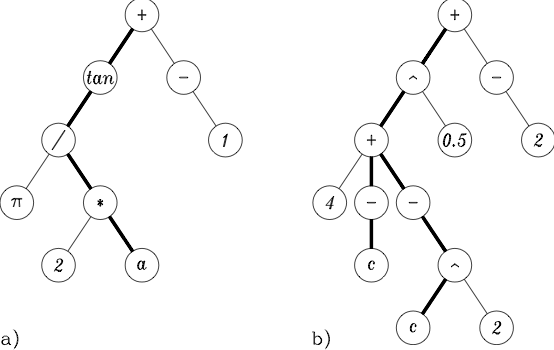
\includegraphics[height=6.4cm]{BAUM.png}
\caption \protect {\begin {minipage} [h] {10cm}% --- TABLE
Tree representation of algebraic expressions
\label{Baum}
\end {minipage}
}%small
\end {center}
\end {figure}
%\inbildpsf{Baumdarstellung algebraischer Ausdr"ucke}{baum.eps}{94mm}{Baum}

An evaluation of the formula complexity regarding the depth of the operation hierarchy, i.e. the degree of the nesting of a term, is now readable at the tree structures. E.g. the complexity can be determined by counting  the branches of a tree, which must be stepped starting from the root of the operation tree, in order to arrive at the instances of the regarded variables.
 In the case of the term in figure \ref{Baum}a) the complexity value $b$ w.r.t. the variable $a$ is equal to the length of the fat drawn path, i.e.\ $b = 4$. In order to achieve all instances of the variable $c$ from the root of the tree in figure  \ref{Baum}b), all in all seven branches must be crossed, therefore the complexity is $b=7$.
 
 This method for the calculation of the complexity is easy expandable in a way, that also the criterion 4 is taken into account, which gives the evaluation of a term regarding the operators contained in it. 
 Instead of the simple counting of the branches of the tree, an additionally weighting must take place, which assigns to each operator an typical "difficulty factor", by which the evaluation of its operands are to be multiplied. The magnitude of this difficulty factor should reflect, how complex the formation of the inverse function for the computer algebra system is, i.e. the solution of the function for its operands, see \cite{Trispel}.

At the beginning each leaf of the tree receives the weighting 1, if it contains that variable, for which the evaluation is to be calculated. Otherwise the leafs get the weighting 0. During the evaluation of the operators the operator  "+" serves as reference for the weighting 1, because it is to be inverted most easily. In contrast, the reversal of the operators  "$*$''  and "$\tan$" are considered arbitrarily as four or ten times as difficulty, accordingly the weightings are set. The following table shows a selection of some operators and their assigned weightings.
\begin{center}
\begin{tabular}{|l|*{7}{c|}}
\hline
operator   & $+$ & $-$ & $*$ & $/$ & $\wedge$ & $\tan$ & $\Arcosh$ \\
\hline
weighting &  1  &  1  &  4  &  4  &    10    &   10   &     12    \\
\hline
\end{tabular}
\end{center}

\begin {figure} [htbp]
\begin {center}
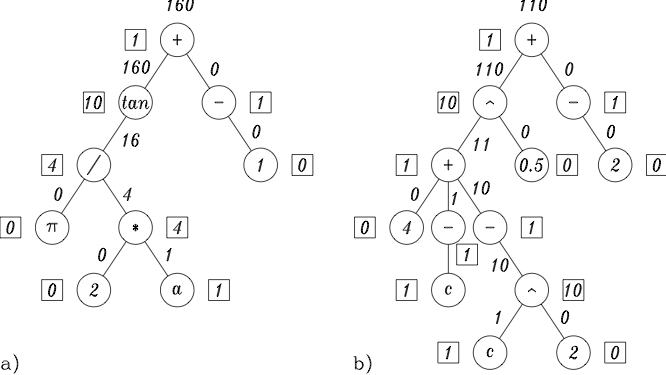
\includegraphics[height=7cm]{BEWERTG.png}
\caption \protect {\begin {minipage} [h] {10cm}% --- TABLE
Valuation of operators
\label{Bewertung}
\end {minipage}
}%small
\end {center}
\end {figure}
%\inbildpsf{Bewertung der Operatoren}{bewertg.eps}{113mm}{Bewertung}

The calculation of the complexity value takes place {\em bottom-up} via repeated addition of the branch weights at the operator nodes, multiplication of this sum with the operator weight and transfer of the resulting value onto the superordinate branch, until the tree root is reached.
 For the demonstration of this procedure the operatior tree in figure \ref{Bewertung}a) is considered. In the squares drawn beside the nodes, the operator weights are marked. The numbers at the branches show the total weight of the subordinated partial tree. Since the complexity of the term is to be evaluated w.r.t. the variable $a$,
only the leaf with the symbol  $a$ gets the weight 1, all other leafs are evaluated with value 0. At the multiplication nodes above the variables, the branch weights add themselves to the sum $0+1=1$, which in accordance with the evaluation of the operator "$*$" are multiplied with the factor 4 and then passed on to right operand branch of  the "$/$" operator. There also takes place a multiplication with 4, so that the intermediate result  now equals to 16. Subsequently, in the process of the calculation  the factors 10 and 1 for the "$\tan$''- and "$+$'' operators are added. The final result, $b=160$, is at the root of the tree. For the operator tree in figure \ref{Bewertung}b) similar calculations result in a complexity value of $b=110$ w.r.t. the variable $c$.

Now, we can take up the temporarily deferred criterion 2. In order to determine those equations of a system, which contain one or more variables at exactly one position, it is sufficient to set all operator weights  in the calculation formula for the term complexity to '1' and to store all pairs of equation/variables, for which under these conditions the complexity evaluation is $b=1$. This method is justified by the fact, that the search aims at exactly those equations, in whose tree representation particular variable symbols occur in only one leaf. 
That means, in these cases there is only one path from the root of the tree  to the symbol in question. With a weighting of '1' for all operators the complexity evaluation  corresponds exactly to the number of paths to the instances of a variable.

This procedure can be verified easily on the basis of examples. If all operator weights are set equal '1', then  for the terms in figure \ref{Bewertung}a) and b) we get complexities of $b=1$ for the variable $a$ and $b=2$ for the variable $c$. This corresponds with the fact, that the variable $a$ is contained in exactly one leaf of the tree, while the symbol $c$ is to be found at two positions.


\subsection{Order of the Sequence of Solution}

By different combining and weighting of the discussed evaluation procedures,   different strategies arise for the order of solution steps. The strategy named \verb+MinVarPathsFirst+, which is implemented in the program developed in this work, represents a combination of the criterion 2 and the complexity evaluation by means of operator weighting. 
Highest priority in the solution step order, receive those equations, which contain wanted variables at exactly one position, whereby within this group one sorts according to smallest weight of the operator trees. 
All remaining pairs of equation/variables are likewise placed to the end of the solution sequence, according to smallest tree weight. 
Therefore in the case of the two terms in figure \ref{Bewertung}, at first it would be  tried to solve the equation with the $\tan$- function for the variable $a$, although  a higher evaluation was calculated for $a$ than for the accompanying term w.r.t. the variable $c$.







